\section{Intro: Integrity to FAIR}
{
    \setbeamertemplate{background canvas}{
        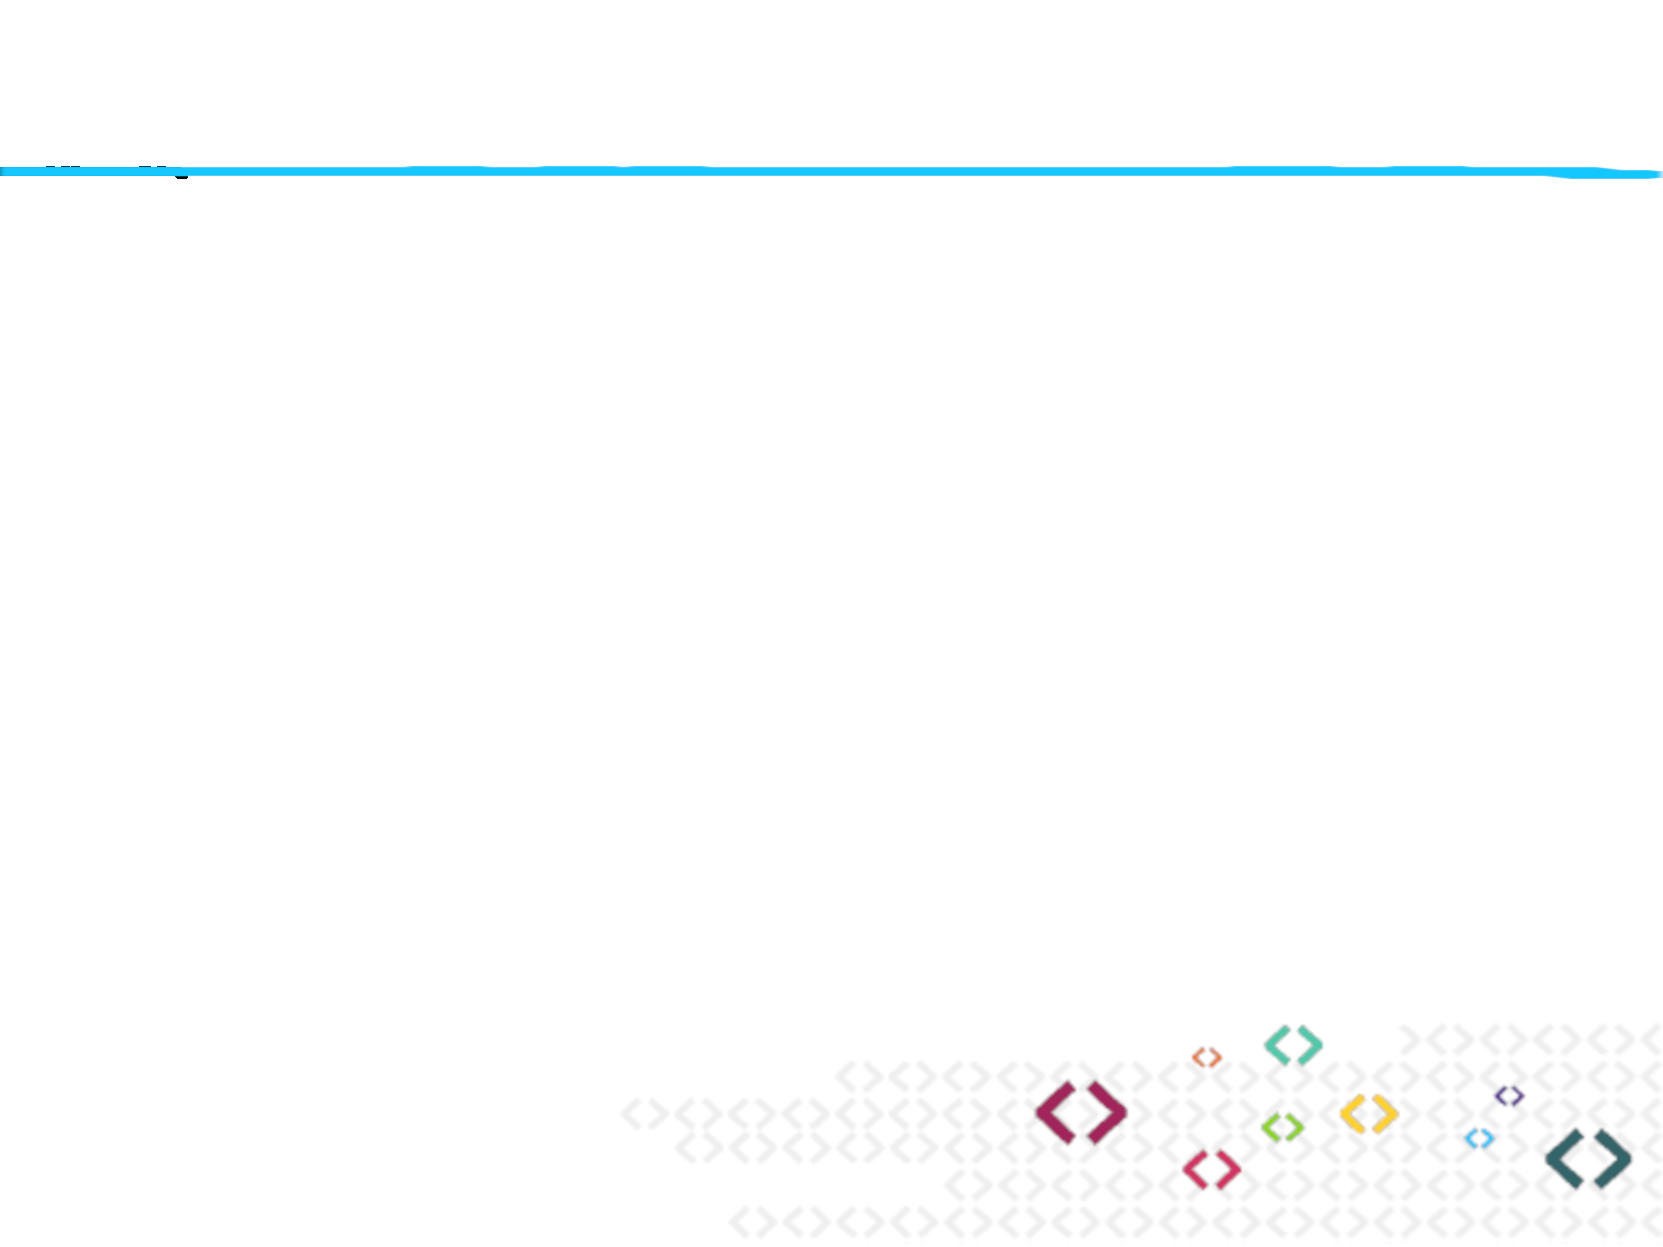
\includegraphics[width=\paperwidth,height=\paperheight]{figs/background_white.png}
    }
    
    \begin{frame}[plain]{Part 1: From Data Integrity to FAIR}{09:15 - 09:45}
        \begin{block}{Goal}
            To connect the foundational, ethical duty of \textbf{Data Integrity} to the modern, practical framework of the \textbf{FAIR Principles}.
        \end{block}
        \begin{center}
            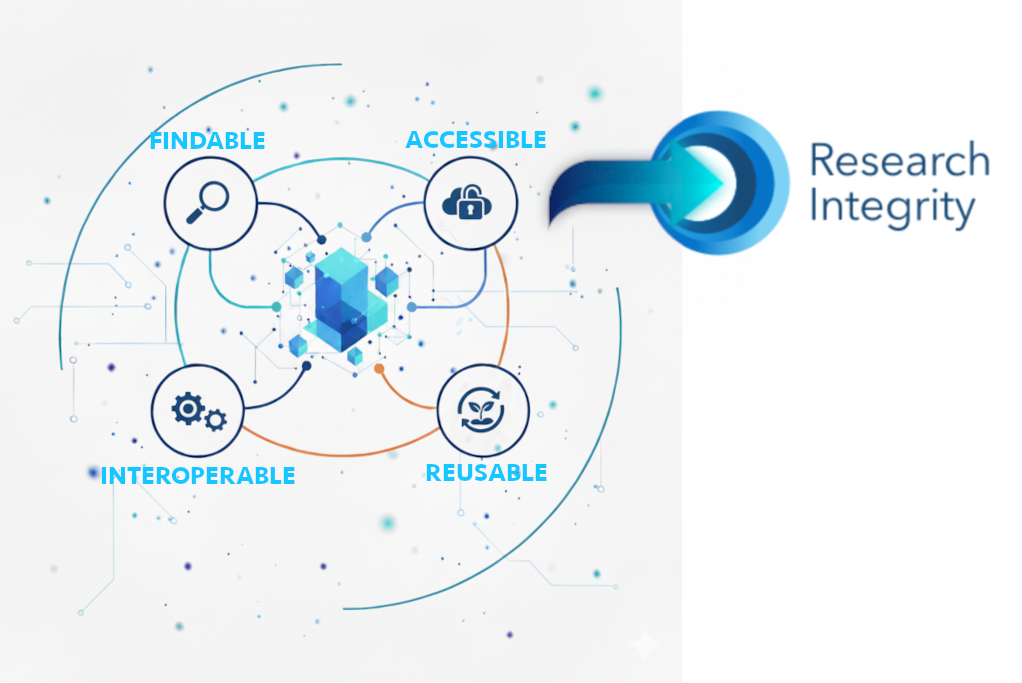
\includegraphics[width=0.56\textwidth]{figs/fig_d1p1/d1p1_01-fairintegrity.png}
        \end{center}
    \end{frame}
}

\begin{frame}{Learning Objectives}
    \begin{itemize}
        \item \textbf{Define} the core concepts of \textbf{Data Integrity} (accuracy, completeness, and consistency) and the four pillars of the \textbf{FAIR} acronym.
        \item \textbf{List} three Guidelines from the DFG code of conduct concerning Data Integrity.
    \end{itemize}
\end{frame}

\begin{frame}{Theory: What is Data Integrity?}{Define}
    \begin{columns}
        \column{.36\textwidth}
        \begin{center}
            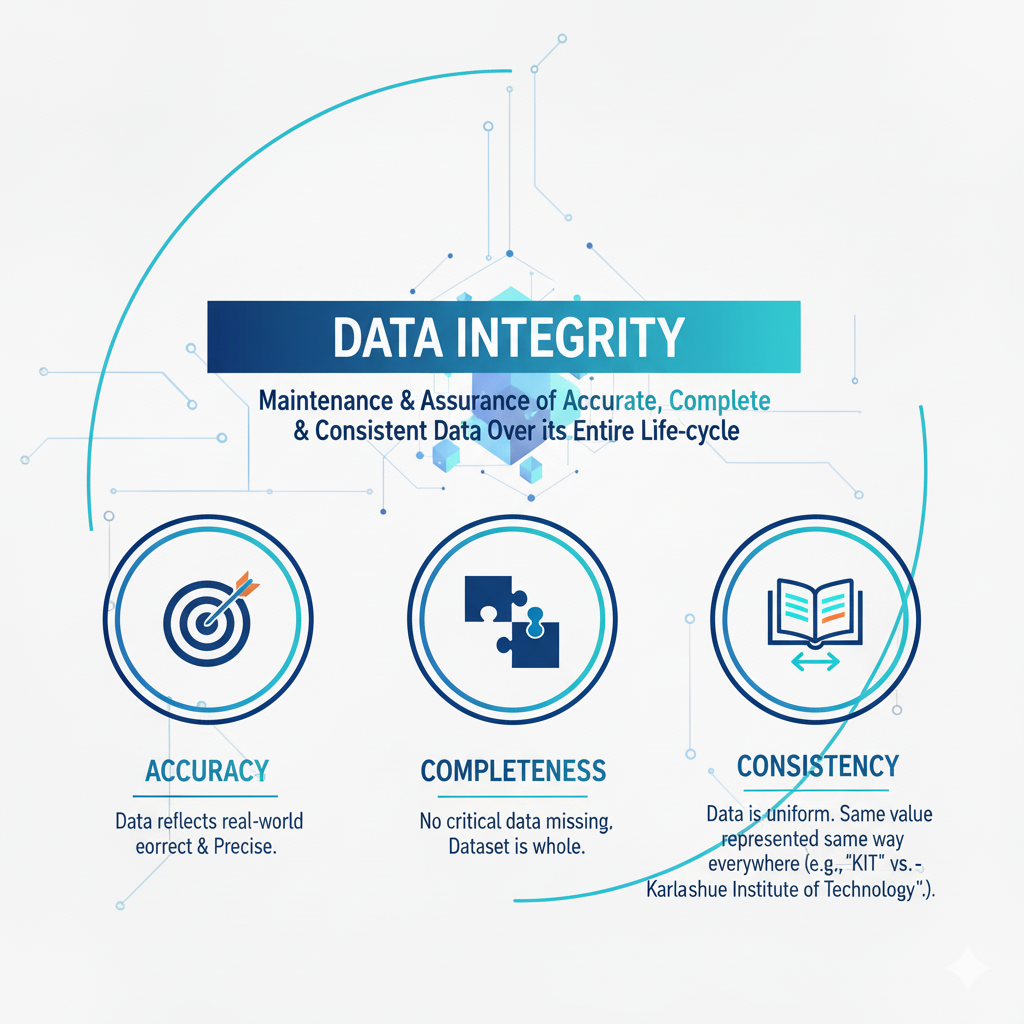
\includegraphics[width=\textwidth]{figs/fig_d1p1/d1p1_02-integrity.png}
        \end{center}
        \column{.64\textwidth}
        \textbf{Data Integrity} is the maintenance and assurance of the \textbf{accuracy}, \textbf{completeness}, and \textbf{consistency} of data over its entire life-cycle.
        \pause
        \begin{itemize}
            \item \textbf{Accuracy:} Data reflects the real-world event. It is correct and precise.
            \pause
            \item \textbf{Completeness:} No critical data is missing. The dataset is whole.
            \pause
            \item \textbf{Consistency:} Data is uniform. The same value is represented the same way everywhere (e.g., `KIT` vs. `Karlsruhe Institute of Technology`).
        \end{itemize}
    \end{columns}
\end{frame}

\begin{frame}{Theory: What are the FAIR Principles?}{Define}
    The FAIR Principles are a set of guiding principles to make research data more valuable and reusable.
    
    \begin{itemize}
        \item \textbf{F}indable: Data (and metadata) must be easy to find by both humans and machines. (e.g., Persistent Identifiers - PIDs).
        \pause
        \item \textbf{A}ccessible: Once found, the (meta)data must be retrievable via a standard protocol. (e.g., HTTP, FTP).
        \pause
        \item \textbf{I}nteroperable: Data must be able to be combined with other datasets, using formal, shared languages and vocabularies.
        \pause
        \item \textbf{R}eusable: Data must be richly described with metadata and have a clear license so it can be replicated or combined.
    \end{itemize}
    More details? \href{https://www.go-fair.org/wp-content/uploads/2022/01/FAIRPrinciples_overview.pdf}{GOFAIR}
\end{frame}

\begin{frame}{Concept: DFG Code of Conduct}{List}
    Data Integrity is a core component of the DFG "Guidelines for Safeguarding Good Research Practice." 
    \cite{deutsche_forschungsgemeinschaft_2025_14281892}
    
    
    \begin{block}{Key Guidelines on Integrity}
        \begin{itemize}
            \item \textbf{Guideline 7 (Safeguarding and Storing):} Researchers safeguard their research data and document the steps taken.
            \pause
            \item \textbf{Guideline 12 (Documentation):} Documentation and re- search results must not be manipulated; they are protected as effectively as possible against manipulation.
            \pause
            \item \textbf{Guideline 17 (Archiving):} Primary data must be securely archived for a minimum of ten years.
        \end{itemize}
    \end{block}
\end{frame}

\begin{frame}{Interactive: Defining Our Terms}{Practice}
    \begin{block}{Group Discussion (8 min)}
        Let's put this together.
        \begin{itemize}
            \item In your own words, what is the biggest threat to \textbf{Data Integrity} in your specific research field?
            \pause
            \item Which of the four \textbf{FAIR} principles do you find the most challenging to implement?
            \pause
            \item How do \textbf{Guideline 12 (\href{https://wissenschaftliche-integritaet.de/en/code-of-conduct/documentation/}{Documentation})} and the 'R' (Reusable) principle relate?
        \end{itemize}
    \end{block}
    \href{https://miro.com/app/board/uXjVJpI_9Kc=/?moveToWidget=3458764648827295133&cot=14}{$\therefore$ Let's miro (How do GRP12 and ’R’ relate)?}
\end{frame}

\begin{frame}{Learning Objectives}
    \begin{itemize}
        \item \textbf{Explain} the \textbf{causal relationship} between maintaining high \textbf{Data Integrity} during collection and achieving the \textbf{Reusability} ('R') principle.
        \item \textbf{Explain} how adhering to the FAIR-Principles is crucial to reach accordance with the DFG guidelines.
    \end{itemize}
\end{frame}

\begin{frame}{Theory: The Integrity-Reusability Chain}{Explain}
    \begin{center}
        \textbf{High Data Integrity} $\rightarrow$ \textbf{Trust} $\rightarrow$ \textbf{Reusability}
    \end{center}
    \vfill
    \begin{itemize}
        \item \textbf{Reusability ('R')} is the ultimate goal of FAIR. It means someone else (or you, in 5 years) can understand, trust, and reuse your data.
        \pause
        \item This is \textbf{impossible} without Data Integrity.
        \pause
        \item If your data is \textbf{inaccurate}, reusing it gives wrong results.
        \item If your data is \textbf{incomplete}, reusing it is impossible.
        \item If your data is \textbf{inconsistent}, reusing it requires massive, error-prone cleaning.
    \end{itemize}
\end{frame}

\begin{frame}{Concept: The Broken Chain}{Explain}
    \begin{block}{Example of Low Integrity}
        A research group publishes a dataset on material strength.
        \begin{itemize}
            \item Column `temp`: Contains values `25C`, `298K`, and `25`.
            \item Column `pressure`: Contains values `1 atm`, `101.3 kPa`, and `1.013`.
        \end{itemize}
        This data is \textbf{inconsistent}.
    \end{block}
    \pause
    \begin{block}{Impact on Reusability}
        A second researcher tries to reuse this data for a meta-analysis. They cannot trust the values. They cannot automate a script. The data is \textbf{not reusable}. The 'R' principle fails.
    \end{block}
\end{frame}

\begin{frame}{Theory: FAIR as a Tool for DFG Concordance}{Explain}
    The DFG Guidelines tell you \textbf{what} to do (e.g., "Archive data", "Document results").
    \pause
    The FAIR Principles tell you \textbf{how} to do it effectively for the modern, digital age.
    
    \begin{itemize}
        \item \textbf{DFG Guideline 7 (Cross-phase quality assurance)} $\rightarrow$ Is achieved by implementing 'R' (Reusable), which requires rich metadata.
        \pause
        \item \textbf{DFG Guideline 12 (Documentation)} $\rightarrow$ Is achieved by implementing domain specific guidelines for assessment and review, along with strong provenance, enabling Interoperability (I).
        \pause
        \item \textbf{DFG Guideline 13 (Providing public access to research results)} $\rightarrow$ Is achieved by implementing 'F' (Findable) with a PID and 'A' (Accessible) in a repository.
    \end{itemize}
    \href{https://miro.com/app/board/uXjVJpI_9Kc=/?moveToWidget=3458764648818228865&cot=14}{$\therefore$ Let's miro (Categories of Metadata for DFG Compliance)?}    
\end{frame}

\begin{frame}{Interactive: The Broken Chain}{Practice}
    \begin{block}{Think-Pair-Share (10 min)}
        \textbf{Scenario:} A researcher leaves KIT. Their raw data is on a USB drive in their desk. The only "documentation" is their published paper.
        \pause
        \textbf{Discuss:}
        \begin{itemize}
            \item Which \textbf{Data Integrity} principles are broken?
            \item Which \textbf{FAIR} principles are broken?
            \item Which \textbf{DFG Guidelines} are broken?
        \end{itemize}
        \pause
        \textbf{Goal:} \textbf{Explain} how these three concepts are deeply linked.
    \end{block}
\end{frame}

\begin{frame}{Learning Objectives}
    \begin{itemize}
        \item \textbf{Apply} data validation and cleaning techniques (e.g., scripting checks, normalisation) to a raw dataset.
        \item \textbf{Write} a checklist to help Researchers assess their own concordance with the guidelines.
    \end{itemize}
\end{frame}

\begin{frame}{Theory: What is Data Validation?}{Apply}
    Data Validation is the set of processes used to ensure data has high \textbf{integrity} (accuracy, completeness, consistency).
    \pause
    \begin{columns}
        \column{.64\textwidth}
        \textbf{Techniques:}
        \begin{itemize}
            \item \textbf{Range Checks:} Is a pH value 15? (Invalid)
            \item \textbf{Format Checks:} Is a date `YYYY-MM-DD`?
            \item \textbf{Normalisation:} Converting all units (C, K) to one standard (K).
            \item \textbf{Schema Validation:} Does the data conform to the rules we set?
        \end{itemize}
        
        \column{.36\textwidth}
        \begin{center}
            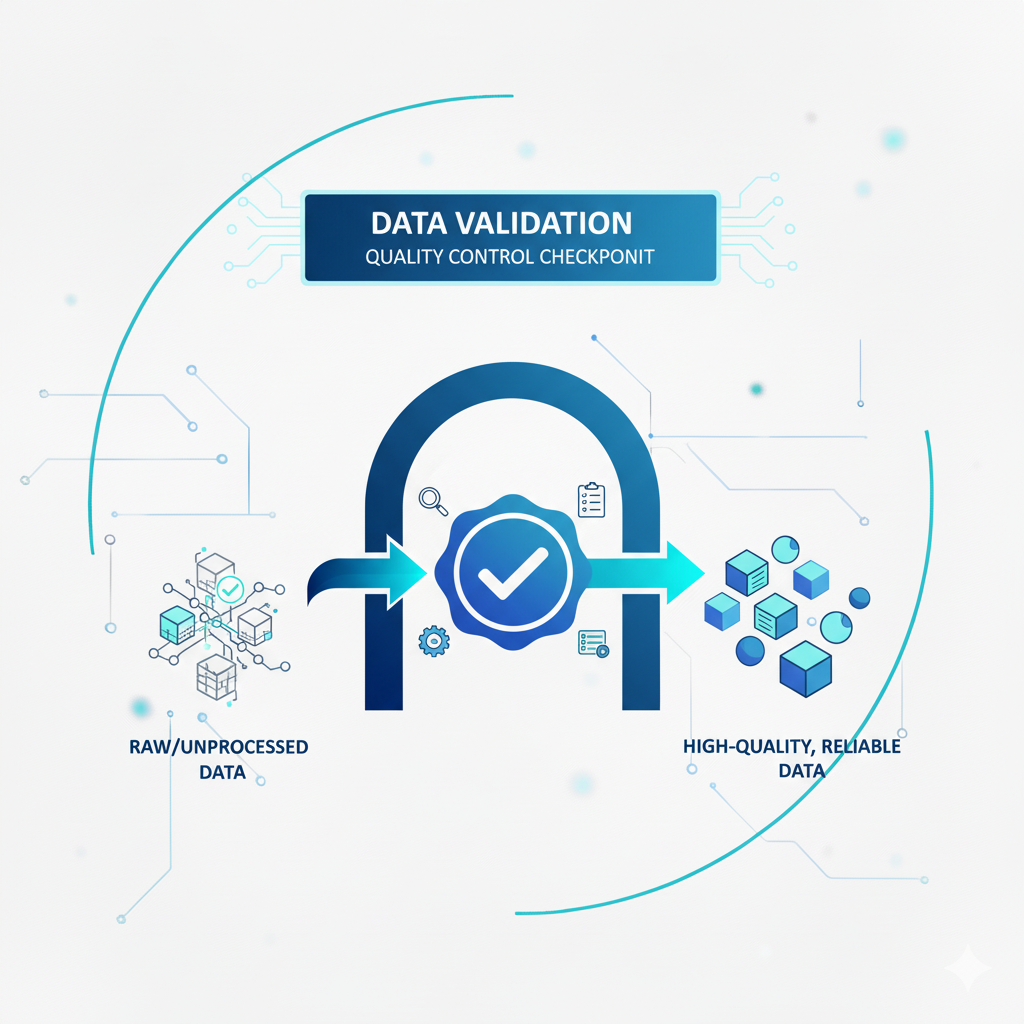
\includegraphics[width=.8\textwidth]{figs/fig_d1p1/d1p1_03-validation_check.png}
            \captionof{figure}{Validation as a Quality Control Checkpoint}
        \end{center}
    \end{columns}
\end{frame}

\begin{frame}[fragile]{Concept: Validation in Practice (Pseudo-Code)}{Apply}
    
    You don't have to check data manually! Use scripts.
    
    \begin{block}{Simple Python Check (Pseudo-code)}
\begin{verbatim}
data = read_csv("my_experiment.csv")
for row in data:
    # Check for completeness (e.g., no missing IDs)
    if row['sample_id'] is None: print("Error: Missing sample_id!")
    # Check for consistency (e.g., standardising units to Kelvin)
    if row['unit'] == "C": row['temp_K'] = convert_to_kelvin(row['temp'])
    # Check for range (e.g., no impossible values below absolute zero)
    if row['temp_K'] < 0: print("Error: Impossible temperature!")
save_csv("my_clean_data.csv", data)
\end{verbatim}
    \end{block}
\end{frame}

\begin{frame}{Interactive: The Concordance Checklist}{Practice}
    \begin{block}{Activity: Write a Checklist (15 min)}
        You are onboarding a new PhD student.
        \pause
        \textbf{Task:} Draft a 5-point "Data Integrity Checklist" to help them assess their own concordance with DFG guidelines.
        \pause
        \begin{itemize}
            \item \emph{Example 1: (Completeness)} "Does every dataset have a `README` file?"
            \item \emph{Example 2: (Consistency)} "Is there a script to check that all units are standardised?"
            \item \emph{Example 3: (Accuracy)} "Has a colleague double-checked the manual data entry?"
        \end{itemize}
        \pause
        \textbf{Goal:} \textbf{Write} this checklist. We will share them.
    \end{block}
    \href{https://miro.com/app/board/uXjVJpI_9Kc=/?moveToWidget=3458764649162553531&cot=14}{$\therefore$ Let's miro (Onboarding)}
\end{frame}

\begin{frame}{Learning Objectives}
    \begin{itemize}
        \item \textbf{Differentiate} between the requirements for data \textbf{Authenticity} (Integrity) and data \textbf{Accessibility} (FAIR).
        \item \textbf{Identify} criteria of publication platforms.
    \end{itemize}
\end{frame}

\begin{frame}{Theory: Authenticity vs. Accessibility}{Differentiate}
    These two concepts are often confused, but are very different.
    
    \begin{columns}
        \column{.5\textwidth}
        \begin{block}{Authenticity (Data Integrity)}
            \textbf{Question:} Is this the \emph{real, unaltered} data?
            \pause
            \textbf{Method:}
            \begin{itemize}
                \item Checksums (e.g., MD5, SHA256)
                \item Digital Signatures
                \item Audit Trails
                \item Version Control History
            \end{itemize}
            \textbf{Metaphor:} A sealed, tamper-proof envelope.
        \end{block}
        
        \column{.5\textwidth}
        \begin{block}{Accessibility (FAIR Principle 'A')}
            \textbf{Question:} Can I \emph{get} to the data?
            \pause
            \textbf{Method:}
            \begin{itemize}
                \item A Persistent Identifier (PID)
                \item A standard protocol (e.g., HTTP)
                \item An open, public URL
                \item Clear authentication (if not open)
            \end{itemize}
            \textbf{Metaphor:} A public mailbox with a clear address.
        \end{block}
    \end{columns}
\end{frame}

\begin{frame}{Concept: PIDs as the Bridge}{Differentiate}
    Persistent Identifiers (like a DOI) are the bridge between Authenticity and Accessibility.
    
    \begin{itemize}
        \item A PID (like a DOI from zenodo) makes the data \textbf{Accessible} ('A') by giving it a permanent,
        findable web address.
        \pause
        \item The repository \textit{behind} the DOI (zenodo) ensures \textbf{Authenticity} (Integrity) by storing the
        file and often providing a checksum (MD5/SHA) to prove it hasn't been altered since publication.
    \end{itemize}
    \pause
    \begin{block}{Key Idea}
        You can have Authenticity without Accessibility (e.g., a file on a secure, offline server).
        \pause
        You should \textit{never} have Accessibility without Authenticity (e.g., a public file that anyone can edit).
    \end{block}
\end{frame}

\begin{frame}{Theory: Criteria for Publication Platforms}{Identify}
    When choosing \textit{where} to publish, you must \textbf{identify} its criteria.
    \begin{itemize}
        \item \textbf{Findability-Degree:} This is key.
        \pause
        \item \textbf{Level 1 (Low):} Publishes data (e.g., a project website).
        \pause
        \item \textbf{Level 2 (Good):} Publishes data + assigns a PID (e.g., KITOpen).
        \pause
        \item \textbf{Level 3 (Excellent):} Publishes data + PID + rich, machine-readable, \emph{domain-specific} metadata (e.g., Open Energy Platform).
    \end{itemize}
    \pause
    \begin{block}{Other Criteria}
        \textbf{Check for:} PID minting (DOIs?), license support (CC-BY?), long-term preservation plan, costs, access control (embargoes?).
    \end{block}
\end{frame}

\begin{frame}{Interactive: Platform Criteria}{Practice}
    \begin{block}{Discussion (10 min)}
        \textbf{Task:} Let's \textbf{identify} criteria for publication platforms.
        \begin{itemize}
            \item What is the "findability-degree" of putting your data on a personal website?
            \pause
            \item What about on a GitHub repository?
            \pause
            \item What about on zenodo?
        \end{itemize}
        \pause
        \textbf{Question:} Why is a high "findability-degree" so important for both you (impact) and your field (progress)?
    \end{block}
    More? \cite{koubaa_energy_2025}
\end{frame}

\begin{frame}{Learning Objectives}
    \begin{itemize}
        \item \textbf{Appraise} a current data storage system against both the criteria for long-term \textbf{Data Security} (Integrity) and \textbf{machine accessibility} ('A' of FAIR).
        \item \textbf{Describe} the importance of the find-ability-degree in selecting where to publish.
    \end{itemize}
\end{frame}

\begin{frame}{Theory: Criteria for Storage vs. Access}{Appraise}
    We must evaluate storage on two axes: Safety (Integrity) and Openness (FAIR).
    
    \begin{columns}
        \column{.5\textwidth}
        \begin{block}{Data Security (Integrity)}
            \textbf{Question:} Is my data safe?
            \begin{itemize}
                \item \textbf{Durability:} Is it backed up?
                \item \textbf{Security:} Who has access?
                \item \textbf{Auditing:} Can I see who changed what? (Version history)
            \end{itemize}
            \begin{center}
                
\includegraphics[width=.24\textwidth]{figs/fig_d1p1/d1p1_04-fortress.png}
            \end{center}
            %\caption{A secure fortress.}
        \end{block}
        
        \column{.5\textwidth}
        \begin{block}{Machine Accessibility ('A')}
            \textbf{Question:} Can a machine get it?
            \begin{itemize}
                \item \textbf{Protocol:} Is it on `http` or `ftp`?
                \item \textbf{Identifier:} Does it have a PID/DOI?
                \item \textbf{Metadata Access:} Is metadata accessible, even if data is restricted?
            \end{itemize}
            \begin{center}
                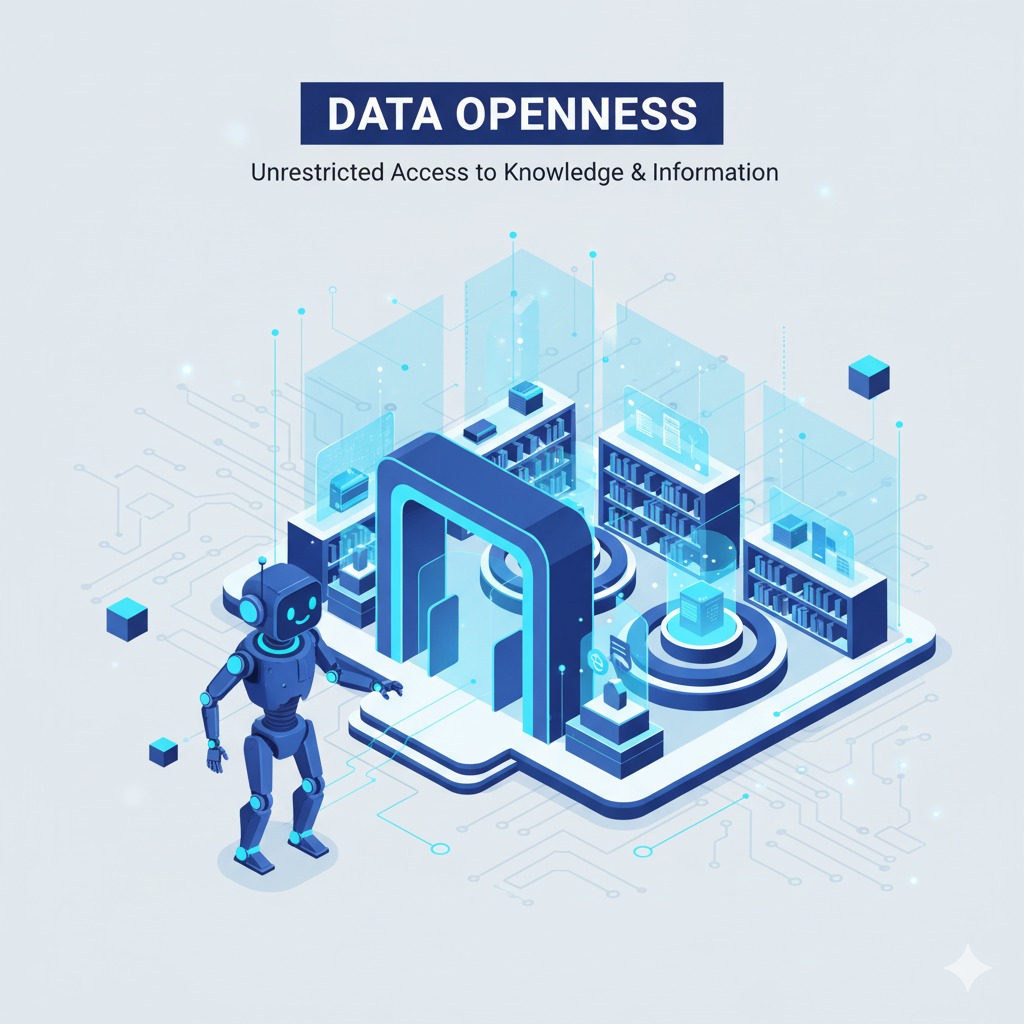
\includegraphics[width=.24\textwidth]{figs/fig_d1p1/d1p1_05-openess.png}
            \end{center}
            %\caption{A robot accessing a library.}
        \end{block}
    \end{columns}
\end{frame}

\begin{frame}{Concept: Evaluating Storage Options}{Appraise Storage Solutions}
    
    Let's appraise common storage systems against our ethical duties.
    \begin{center}
        \begin{tabular}{p{0.24\textwidth}|p{0.33\textwidth}|p{0.33\textwidth}}
            \toprule
            \textbf{Storage System} & \textbf{Data Security (Integrity)} & \textbf{Machine Access ('A')} \\
            \midrule
            
            % Use \pause immediately before the text to be revealed
            \pause
            Your Laptop HD & \textcolor{HMCBlue!40}{\textbf{Very Low}\newline (No backup, easily lost)} & \textcolor{HMCBlue!20}{\textbf{None}\newline (Offline)} \\
            \addlinespace
            
            % \pause is now used only at the start of the row to make the whole row appear.
            \pause
            Shared Drive & \textcolor{HMCBlue!80}{\textbf{Medium}\newline (Backed up, access control)} & \textcolor{HMCBlue!60}{\textbf{Low}\newline (Internal, not public)} \\
            \addlinespace
            
            \pause
            GitHub (Public) & \textcolor{HMCBlue}{\textbf{High}\newline (Versioned, backed up)} & \textcolor{HMCBlue!80}{\textbf{Medium}\newline (No PID, not a formal repo.)} \\
            \addlinespace
            
            \pause
            KITOpen (Repo.) & \textbf{Very High}\newline (Managed, backed up) & \textbf{Very High}\newline (Public, HTTP, PID) \\
            \bottomrule
        \end{tabular}
    \end{center}
\end{frame}

\begin{frame}{Interactive: Appraise Your Storage}{Practice}
    \begin{block}{Personal Evaluation (10 min)}
        \textbf{Task:} Think about the \emph{primary} place you store your "in-progress" research data right now.
        \begin{itemize}
            \item \textbf{Appraise} its \textbf{Data Security}. What is your biggest risk? (e.g., "My laptop gets stolen," "A colleague overwrites the file.")
            \pause
            \item \textbf{Appraise} its \textbf{Machine Accessibility}. Could an external collaborator (or a script) access it without you emailing it?
        \end{itemize}
        \pause
        \textbf{Share:} Let's hear some examples.
    \end{block}
\end{frame}

\begin{frame}{Learning Objectives}
    \begin{itemize}
        \item \textbf{Develop} a comprehensive, integrity-focused \textbf{Metadata Standard} that, when implemented, ensures the data meets all FAIR principles.
        \item \textbf{Distinguish} different types of interoperability (The 5 Stars).
    \end{itemize}
\end{frame}

\begin{frame}{Theory: What is a Metadata Standard?}{Develop}

    A Metadata Standard is not just a list of fields. It's a complete \textbf{"instruction manual"} for your data, essential for maintaining data integrity (\href{https://github.com/OpenEnergyPlatform/oemetadata}{an example?}).

    It must define:
    \begin{enumerate}
        \pause
        \item \textbf{Schema:} What fields are required? (e.g., \texttt{Creator}, \texttt{Date}, \texttt{Sample\_ID}).
        \pause
        \item \textbf{Vocabularies:} What are the allowed \textit{values} for a field? (e.g., For \texttt{Unit}, you must use \texttt{K}, \texttt{m}, or \texttt{kg}. No \texttt{Celsius} or \texttt{grams}.)
        \pause
        \item \textbf{Format:} How is it written? (e.g., "All metadata will be stored as a \texttt{metadata.json} file alongside the data.")
    \end{enumerate}
    \pause
    \begin{block}{Key Idea}
        An "integrity-focused" standard \textbf{requires} fields that ensure accuracy (e.g., \texttt{Instrument\_Calibration\_Date}) and consistency (e.g., \texttt{Unit\_Standard}).
    \end{block}
\end{frame}

\begin{frame}{Concept: The 5 Stars of Interoperability}{Distinguish}
    \begin{columns}
        
    \column{.36\textwidth}
    \begin{center}
        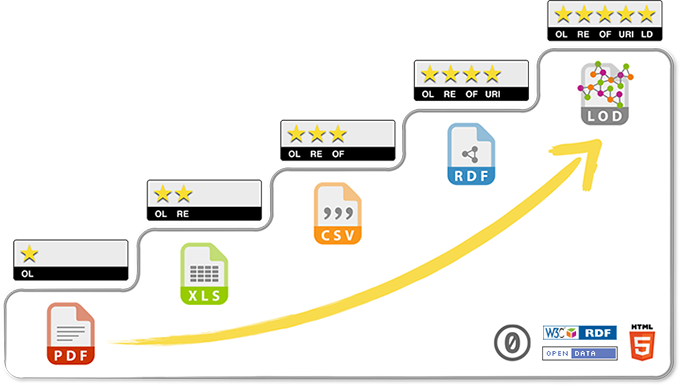
\includegraphics[width=\textwidth]{figs/fig_d1p1/5-star-steps.png} \cite{BernersLee5StarData}
    \end{center}
    \column{.64\textwidth}
    \begin{itemize}
        \item $\star$ -- Data is on the web (e.g., a PDF)
        \item $\star\star$ -- Machine-readable (e.g., an Excel file)
        \item $\star\star\star$ -- Non-proprietary format (e.g., a CSV file)
        \item $\star\star\star\star$ -- Uses URIs/PIDs as identifiers
        \item $\star\star\star\star\star$ -- \textbf{Links} to other data (Linked Open Data)
    \end{itemize}
    \pause
    This is the \href{https://5stardata.info/en/}{$\therefore$ ladder} we are trying to climb!
    \end{columns}
\end{frame}

\begin{frame}{Interactive: Brainstorm Your Standard}{Practice}
    \begin{block}{Workshop (8 min)}
        \textbf{Task:} Let's \textbf{develop} a \textit{minimal} metadata standard for a simple experiment.
        \pause
        \textbf{Scenario:} Measuring the temperature of 10 water samples.
        \pause
        \textbf{Brainstorm:} What fields are \textit{essential} for...
        \begin{itemize}
            % Fix: Escaping underscores with \_ within the \texttt{} environment
            \item \textbf{Integrity:} (e.g., \texttt{operator\_{name}}, \texttt{calibration\_{date}})
            \item \textbf{FAIRness:} (e.g., \texttt{sample\_{id}}, \texttt{unit}, \texttt{location\_{geocoordinates}})
        \end{itemize}
        \pause
        \textbf{Goal:} \textbf{Distinguish} between fields for simple documentation and fields for 5-star interoperability.
    \end{block}
    \href{https://miro.com/app/board/uXjVJpI_9Kc=/?moveToWidget=3458764649160876023&cot=14}{$\therefore$ Let's miro (temperature of 10 water samples)}
\end{frame}

\begin{frame}{Summary}
    \begin{itemize}
        \item \textbf{Data Integrity} (Accurate, Complete, Consistent) is the foundation.
        \item \textbf{FAIR Principles} are the practical framework for modern data.
        \item \textbf{DFG Guidelines} are the "law" that requires both.
        \item We apply integrity by \textbf{validation} and \textbf{appraising} our tools.
        \item We plan for FAIR by developing \textbf{Metadata Standards}.
        \item RDA Guidelines for publishing structured metadata on the web \cite{wu_2021_5727048} can be considered.
    \end{itemize}
    \vfill
    \begin{center}
        \textbf{End of Part 1}
    \end{center}
\end{frame}

\begin{frame}{Bibliography}
    \printbibliography
\end{frame}